\documentclass{beamer}
\setbeamertemplate{navigation symbols}{}%屏蔽右下角引导符
\usetheme{Warsaw}
%\useinnertheme{rectangles}%矩形框
\useinnertheme{circles}
\useoutertheme{infolines}
\useoutertheme[title,section,subsection=true]{smoothbars}



\usepackage{
	amsmath,			% 数学环境
	amssymb,			% 扩展符号
	enumerate,		    % 枚举环境
	graphicx,			% 包含图片
	lastpage,			% 参考资料
	multicol,			% 使用多列
	multirow,			% 使用多行
	pifont,			    % 复选标记
	booktabs,        %Allows the use of \toprule, \midrule and \bottomrule in tables
	stmaryrd			% For brackets
}
\usepackage[english]{babel}
\usepackage[UTF8,noindent]{ctexcap}



\definecolor{2}{RGB}{95,28,39}%星际牛仔
\definecolor{1}{RGB}{28,50,100}
%\definecolor{1}{RGB}{255,151,0}%p站配色
%\definecolor{2}{RGB}{0,0,0}
%\definecolor{1}{RGB}{79,78,119}%星际牛仔spike配色
%\definecolor{2}{RGB}{240,230,90}

\setbeamercolor{title}{fg=2}
\setbeamercolor{frametitle}{fg=1}
\setbeamercolor{structure}{fg=1}
\setbeamercolor{section in head/foot}{bg=2}
\setbeamercolor{author in head/foot}{bg=2}
\setbeamercolor{date in head/foot}{fg=2}
\setbeamercolor{structure}{fg=1}
\setbeamercolor{local structure}{fg=black}
\beamersetuncovermixins{\opaqueness<1>{0}}{\opaqueness<2->{15}}
%\definecolor{UniOrange}{RGB}{212,69,0}
%\definecolor{UniGray}{RGB}{62,61,60}
%%\definecolor{UniRed}{HTML}{B31B1B}
%%\definecolor{UniGray}{HTML}{222222}
%\setbeamercolor{title}{fg=UniGray}
%\setbeamercolor{frametitle}{fg=UniOrange}
%\setbeamercolor{structure}{fg=UniOrange}
%\setbeamercolor{section in head/foot}{bg=UniGray}
%\setbeamercolor{author in head/foot}{bg=UniGray}
%\setbeamercolor{date in head/foot}{fg=UniGray}
%\setbeamercolor{structure}{fg=UniOrange}
%\setbeamercolor{local structure}{fg=black}
%\beamersetuncovermixins{\opaqueness<1>{0}}{\opaqueness<2->{15}}


\useinnertheme{default}
\usefonttheme{serif}
\usepackage{palatino}
\setbeamerfont{title like}{shape=\scshape}
\setbeamerfont{frametitle}{shape=\scshape}
\setbeamertemplate{itemize items}[circle]%无序列表
\setbeamertemplate{enumerate items}[default]%有序列表



%\newcommand{\N}{\mathbb{N}}
%\newcommand{\Z}{\mathbb{Z}}
%\newcommand{\Q}{\mathbb{Q}}
%\newcommand{\R}{\mathbb{R}}
%\newcommand{\C}{\mathbb{C}}



\DeclareMathOperator{\im}{im}
\DeclareMathOperator{\Span}{span}



%\newcommand{\pf}{\noindent\emph{Proof. }}
\newcommand{\ds}{\displaystyle}
\newcommand{\defeq}{\stackrel{\text{def}}{=}}
\newcommand{\ov}[1]{\overline{#1}}
\newcommand{\ma}[1]{\stackrel{#1}{\longrightarrow}}
\newcommand{\twomatrix}[4]{\begin{pmatrix} #1 & #2 \\ #3 & #4 \end{pmatrix}}



\usepackage{tikz}
\usepackage{tikz-cd}
\usetikzlibrary{
	calc,
	decorations.pathmorphing,
	matrix,arrows,
	positioning,
	shapes.geometric
}
\usepackage{pgfplots}
\pgfplotsset{compat=newest}



%\theoremstyle{plain}
%\newtheorem{thm}{Theorem}[section]
%\newtheorem{prop}{Proposition}[section]
%\newtheorem{lem}{Lemma}[section]
%\newtheorem{cor}{Corollary}[section]
\theoremstyle{definition}
%\newtheorem{ex}{Example}[section]
%\newtheorem{nex}{Non-Example}[section]
\newtheorem{框}{框框}[section]
%\theoremstyle{remark}
%\newtheorem{rem}{Remark}[section] 
\numberwithin{equation}{section}




% -------------------
% 标题页
% -------------------
\title{\textcolor{white}{这\ 是\ 标\ 题}}
\subtitle{\textcolor{white}{这\ 是\ 小\ 标\ 题\ 小\ 标\ 题}}  
\author{某\ 某\\ 1111111}
\date{\today} 


% -------------------
% 内容
% -------------------
%\setbeamertemplate{bibliography item}[text]
\begin{document}
	
	
	\begin{frame}
		\titlepage
	\end{frame}
	
	
	
	\section{第一个内容}
	
	
	
	 
	\begin{frame}
		这就是第一个内容 \dots
	\end{frame}
	
	
	
	\begin{frame}
		这是第一个剩下的内容 \dots
		
		\begin{框}[说点什么]
			框框里的话
		\end{框}
		
		\begin{框}
			话话话话 \emph{qiang diao}.
		\end{框}
	\end{frame}
	
	
	
	% Main Results
	\section{第二个内容}
	
	
	
	% Theorem
	\begin{frame}
		\begin{框}[一些话]
			For all $n$, we have $n^2= n \cdot n$.
		\end{框}
		
		pf With massive loss of generality, let $n=1$. Then we have
		\[
		1=1^2= 1 \cdot 1= 1
		\]
		Therefore by overwhelming hope, it must always be true. \qed
	\end{frame}
	
	
	

	\begin{frame}
		Most algebra you need to be true is true.
		\begin{框}
			For all $n,m \in N$, $(n+m)^2= n^2 + m^2$.
		\end{框}
	\end{frame}
	
	
	
	\section{三}
	
	
	
	% 三 1
	\begin{frame}
		\begin{enumerate}[1.]
			\item Bleach is mostly water. \pause
			\item We are mostly water. \pause
			\item Therefore, we are bleach.
		\end{enumerate} \vspace{0.5cm}
		
		Now we pause for the big reveal\dots \pause \vspace{0.3cm}
		
		\begin{itemize}
			\item I am clearly a master of logic.
			\item Masters of logic get Ph.D's.
			\item I have earned this.
		\end{itemize}
	\end{frame}
	
	
	

	\begin{frame}
		Finally! Some Math! \vspace{1cm}
		
		Here is some Math: $\int_1^\alpha \dfrac{x^2}{\sin x^2} \;dx$ and $\sum i^2$. \vspace{1cm}
		
		But you could make this Math big inline with `displaystyle': $\ds \int_1^\alpha \dfrac{x^2}{\sin x^2} \;dx$ and $\ds \sum i^2$. \vspace{1cm}
		
		And even more Math:
		\[
		\oint \vec{\nabla} \times \vec{F} \;dV = \sum_{n=1}^\infty \ov{p} \twomatrix{a}{b}{c}{d}
		\]
	\end{frame}
	
	
	
	\section{Conclusion}
	
	
	
	\begin{frame}
		Ph.D. plz\dots
	\end{frame}


    \begin{frame}
    	\frametitle{Figure}
    	\begin{center}
    		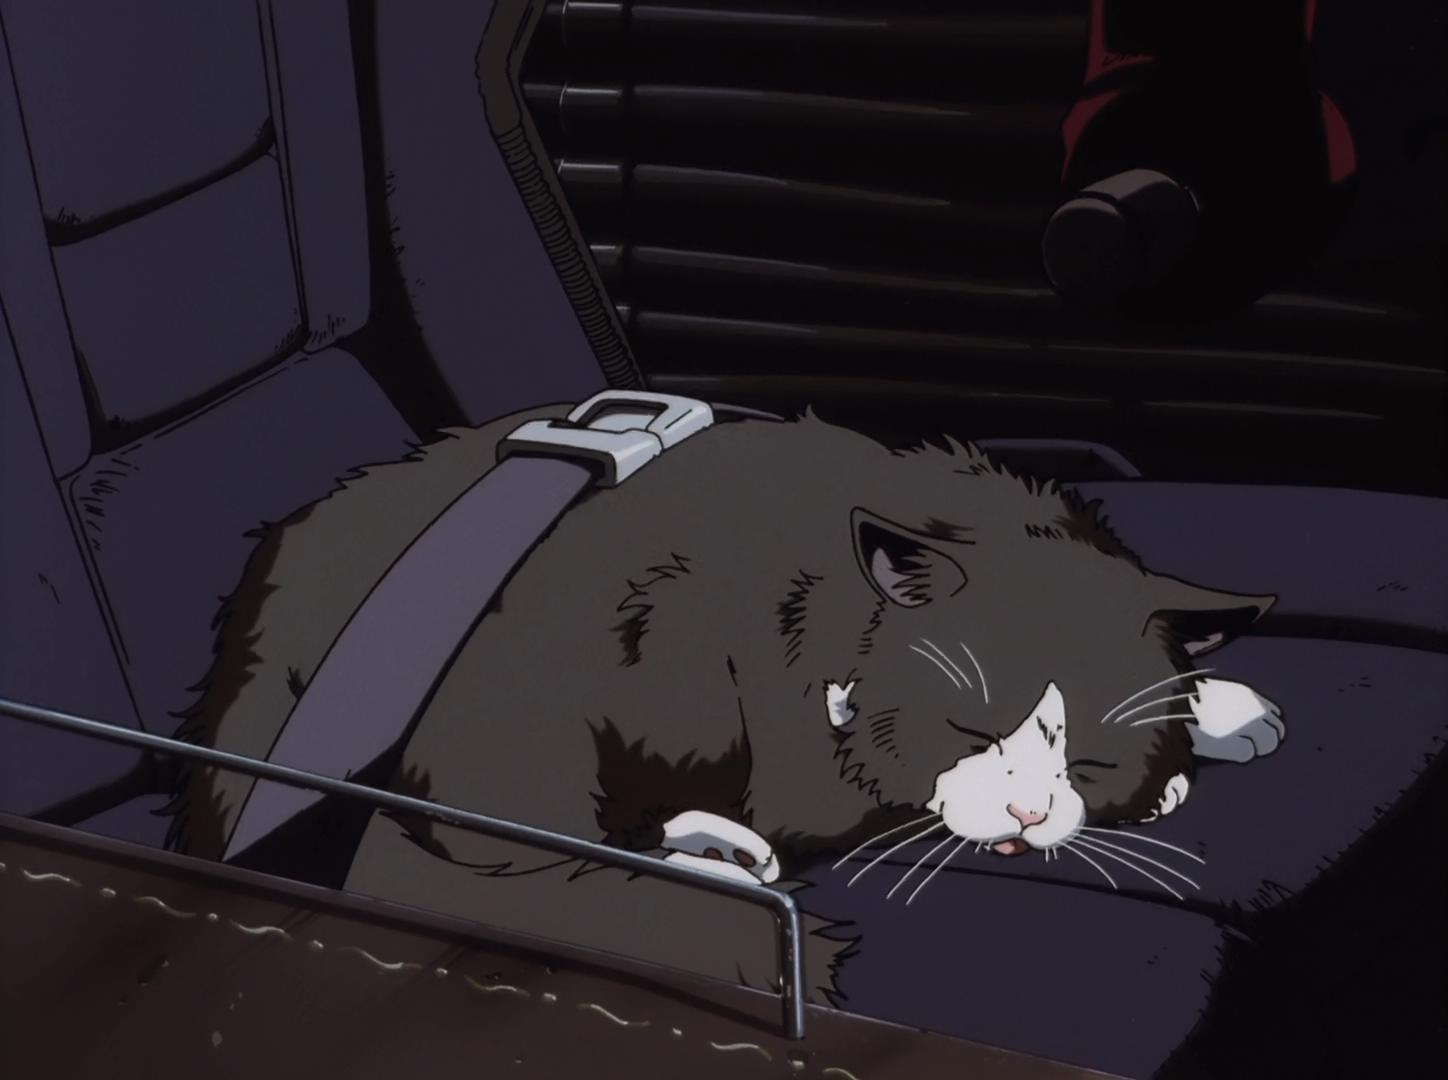
\includegraphics[width=0.5\linewidth]{./image/test}    %插入图片
    		%\includegraphics[width=1.0\linewidth]{1}
    	\end{center}
    \end{frame}



    \begin{frame}
    	\frametitle{Table}
    	\begin{table}
    		\begin{tabular}{l l l}
    			\toprule
    			\textbf{Treatments} & \textbf{Response 1} & \textbf{Response 2}\\
    			\midrule
    			Treatment 1 & 0.0003262 & 0.562 \\
    			Treatment 2 & 0.0015681 & 0.910 \\
    			Treatment 3 & 0.0009271 & 0.296 \\
    			\bottomrule
    		\end{tabular}
    	    \caption{Table caption}
       \end{table}
    \end{frame}
	
	
	
	\begin{frame}
		\frametitle{References}
		\footnotesize{
			\begin{thebibliography}{99} % Beamer不支持BibTeX,因此必须手动插入引用,如下所示。
				\bibitem[Smith, 2012]{p1} John Smith (2012)
				\newblock Title of the publication
				\newblock \emph{Journal Name} 12(3), 45 -- 678.
			\end{thebibliography}
		}
	\end{frame}
	
	
	
	\begin{frame}
		\begin{center} {\bfseries \Large 谢\ 谢!} \end{center}
	\end{frame}
	
	
\end{document}
